Cartographic visualizations are the interface between the GIS and the human. A map is is the common form. It is a discrete graphical expression of the continuous real world. The creation of a map is not just a scientific, but also a creative process: The form, function and interaction methods shall follow the purpose of the usage of the map.

There is no fixed guideline how to properly design a map, but there are typical elements that are part of every cartographic visualization.The main element is the map itself, using a specific map projection
% (see section \ref{ssub:map_projections})
, a scale and an initial center point. A map is typically structured in a \emph{layer} principle. Each layer is a transparent film showing one specific aspect, e.g. a physical layer showing coastlines, mountains or forests, a political layer showing international borders or a cultural layer showing cities or population densities. The layers are interchangeable, can be switched on and off and serve to serve a different visualization purpose. The map is designed using a certain color scheme, fonts and signatures for all the objects on the map.

Additionally there can be a \emph{title} describing the purpose of the map. A \emph{legend} including the scale bar and north arrow shall explain all symbols used on the map and give orientation. Depending on the degree of interactivity, there can be \emph{menus} with different visualization options, e.g. panning and zooming on the map, switching map layers on and off or changing the color scheme of the map.
\cite[pp. 159-166]{bolstad2008gis}

% example of a good map

The main goal of map design is to give the user nothing but the necessary information he needs to satisfy his or her information need. The cartographer shall use techniques of \emph{cartographic generalization} to minimize information on the map and maximize the knowledge to be extracted from the map. Simplification, smoothing or aggregation help to reduce amount of information. Enlarging, widening or displacement help to focus on the important areas of the map. Selection and classification help the user to get an overview of the information.
\cite{krygier2005making}

Leaflet.js is ``an open-source JavaScript library for mobile-friendly interactive maps''
\footnote{
  \textit{Leaflet - JavaScript library for interactive maps},
  URL: \url{http://leafletjs.com/},
  last access: 02.11.2015
}
that offers functionality to embed a map with a chosen projection in an HTML document, use own map tiles, symbols and markers on the map and tools for zooming and panning.
The same service is provided by \emph{OpenLayers}, a ``A high-performance, feature-packed library for all your mapping needs''
\footnote{
  \textit{OpenLayers 3 - Welcome},
  URL: \url{http://openlayers.org/},
  last access: 02.11.2015
}, just with more features and users.


% ------------------------------------------------------------------------------
\subsubsection{Maps} % (fold)
\label{ssub:maps}


maps are means and products of GIS

scientific visualization vs. information visualization
  tangible objects            abstract concepts
  with inherent form          without inherent form
  e.g. CT scan of human body  e.g. flow of refugees
-> 3D globe: inherent form, direct representation of Earth -> scientific visualization
-> 2D map and time: no inherent form resp. abstract concept
=> information visualization

tasks of visualization
  present (what? where? when? how?)
  analyze (e.g. what is the best? where is the most? when was the first?)
  explore (why?)
% \cite Kraak 1999

interactive map enhances human cognition (panning, zooming, changing map layers, time point, data source, ...) and lets him gain knowledge about the domain

maps contain symbols and elements
  ... blaaa ...

traditional paper maps vs. modern digital maps
\begin{table}[ht]
\centering
\begin{tabular}{llp{1em}ll}
    \toprule
    \multicolumn{2}{c}{classical map} & & \multicolumn{2}{c}{modern digital map} \\
    character & restriction & & character & improvement \\
    \midrule
    static & only discrete point in time & & dynamic & higher sample rate for continuous processes \\
    isolating & only part of geographical space in 2D & & multi-dimensional & multiple levels of detail, possibility for representation of elevation and temporal dimension \\
    selective & only one layer & & inclusive & change layers and perspectives \\
    passive & only sending information & & interactive & direct manipulation and exploration \\
    \bottomrule
\end{tabular}
\caption{Innovation of modern digital maps}
\small{alternation of \cite{karcher} and \cite[p. 145]{ott2001time}}
\label{tab:maps_restrictions}
\end{table}

modern digital maps can show changes in time and space due to their dynamic, multi-dimensional, inclusive and interactive nature.


\paragraph{Map Projections} % (fold)
\label{par:map_projections}

One task of a HGIS is to visualize the Earth on a map. Since the Earth is an inhomogeneous three-dimensional shape but the output medium is a two-dimensional computer screen or piece of paper, it has to be transformed.

Based on the geodetic datum a three-dimensional representation of the Earth in form of a globe would be a possible medium to view the planet. When seen perpendicular onto the world, a globe represents sizes, shapes, distances and directions of objects close to the viewpoint with a reasonable accuracy. However, they are very space-consuming and cumbersome. For a precise measurement of distances, following a route or examining a terrain model, the globe would have to be very large. Therefore, the desired medium for practical purposes is a two-dimensional map.

The basic problem to be solved is that the Earth is a spherical object, its surface is curved and it is therefore not straightforward to project it onto a flat 2D map. The meridians which are lines of equal value converge at the poles. Neighboring meridians (distance: 1\degree) have a distance of 111 km at the Equator and 0 km at the poles. They do not form a right-angled grid with the parallels and therefore no Cartesian coordinate system. This is the reason why the geometries of the spherical Earth will be distorted when displayed on a flat 2D Cartesian coordinate system. \cite[p.79]{bolstad2008gis}

% \begin{figure}[ht]
%   \centering
%   \includegraphics[width=0.66\textwidth]{graphics/basics/distortion}
%   \caption{Distortion visualized by circles on a 2D map as a Cartesian coordinate system}
%   (on the 3D Earth all circles have the same size)
%   \label{fig:distortion}
% \end{figure}

There are two main classifications of map projections: The \emph{projection family} with respect to the geometric shape used for the transformation: \emph{cylindrical}, \emph{conical} and \emph{azimuthal} or \emph{planar projection}). Secondly, the \emph{distortion characteristics} with respect to the map property that is preserved. There are \emph{equivalent}, \emph{conformal}, \emph{equidistant}, \emph{zenithal} and compromise projections. Most families and characteristics can be mixed, e.g. it is possible to create a cylindrical, a conical and an azimuthal equivalent map projection
\cite{mapProjectionKrygier}.


\paragraph{Projection Families} % (fold)
\label{subp:projection_families}

The basis of geometrical map projections are \emph{developable surfaces} onto which the ellipsoidal model of the Earth is projected. The are mainly three geometric shapes that are used as reference surfaces: cylinders, cones and planes. The model is fitted in or on the surface touching it in at least one point or line. The idea is that there is a projection source from which rays are shot through the ellipsoid on the surface, projecting each point of the ellipsoid onto the surface (as seen in figure \ref{fig:projections}). This principle is known from the ray casting technique in computer graphics
\cite{mapProjectionGeokov}.

\begin{figure}[ht]
  \centering
  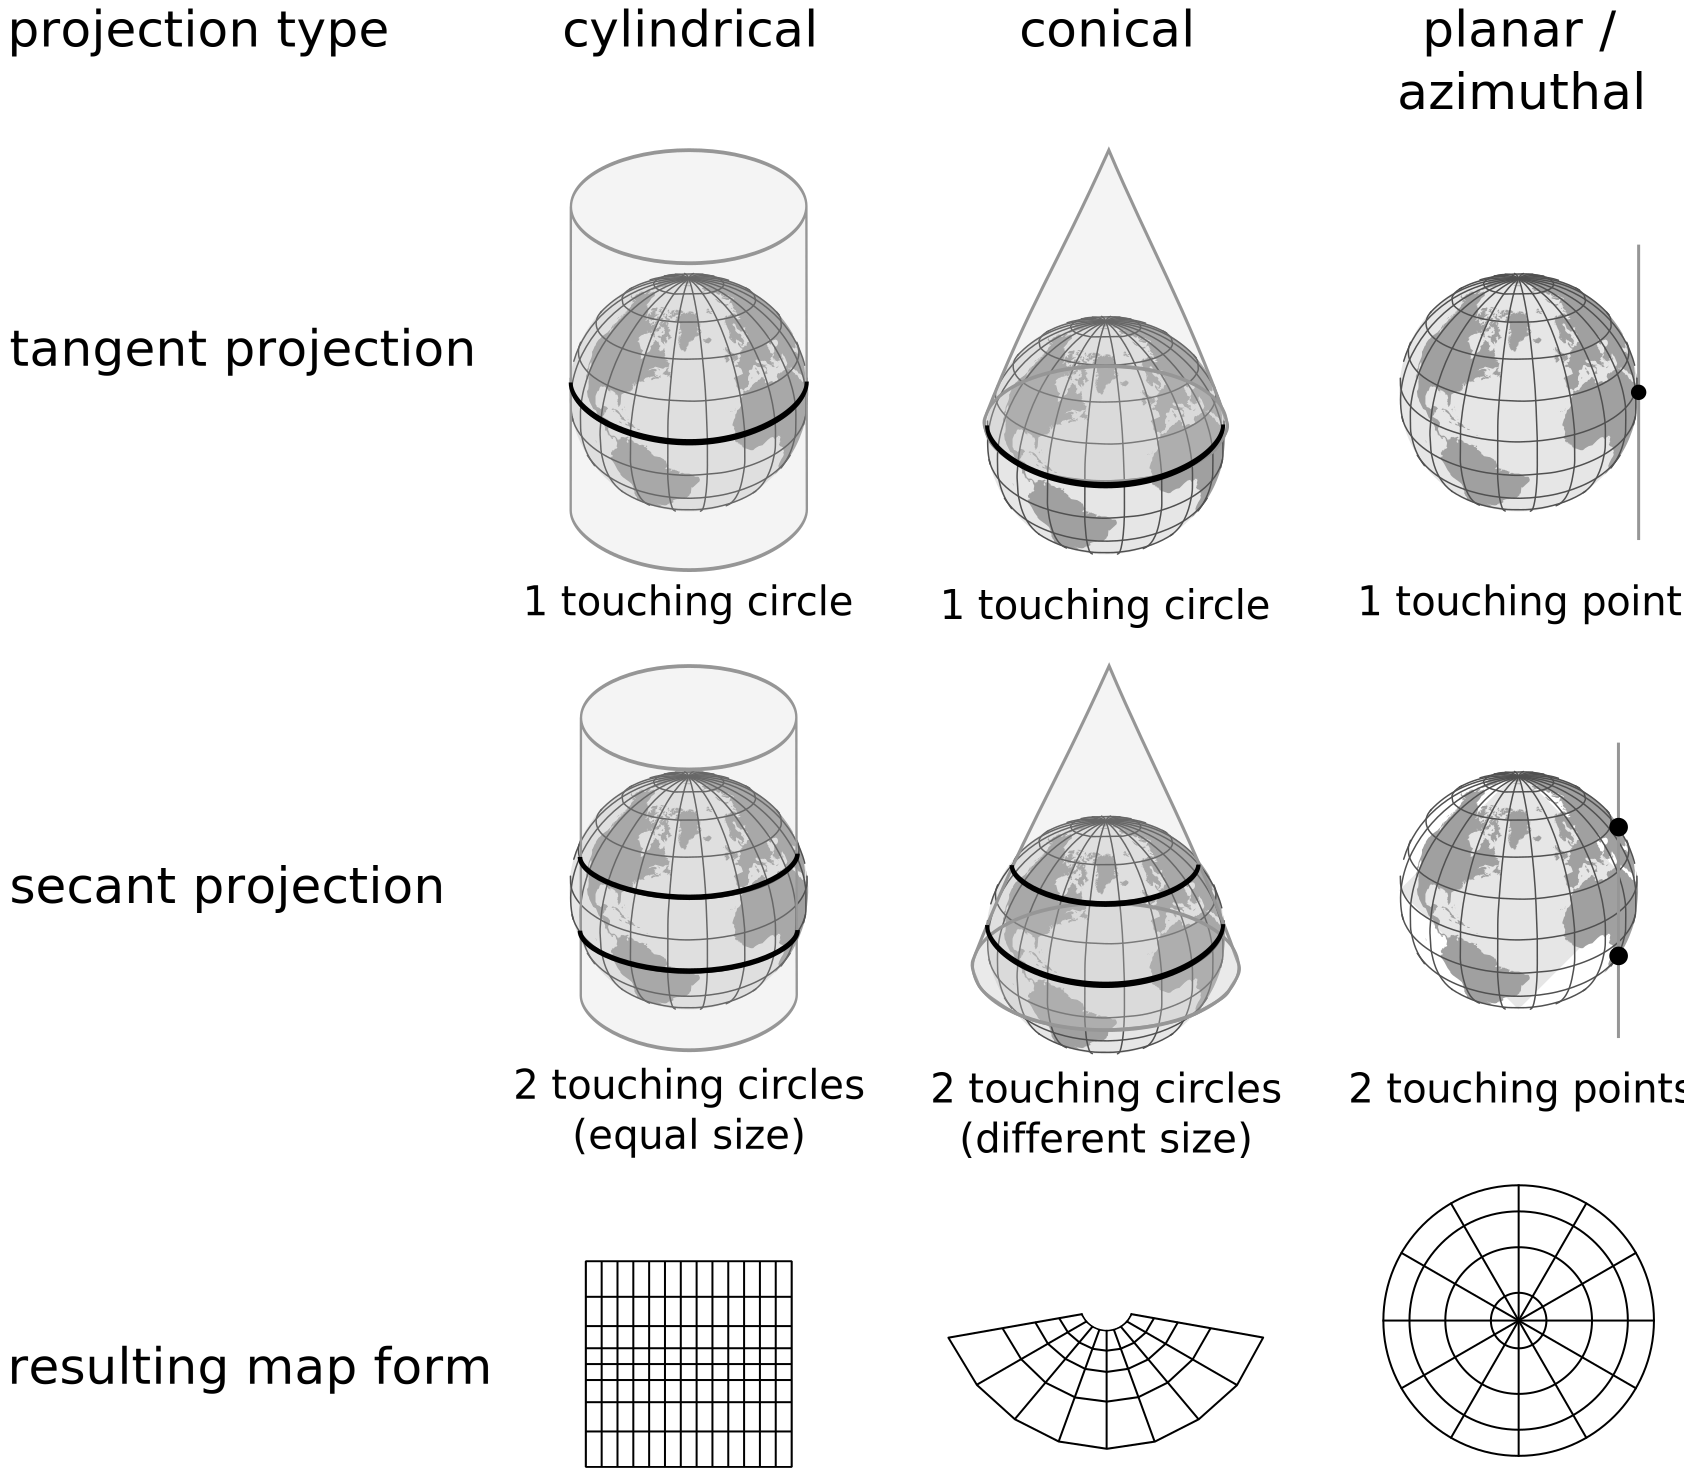
\includegraphics[width=0.73\textwidth]{graphics/basics/projections}
  \caption{Three different developable surfaces for map projections \protect\footnotemark}
  \label{fig:projections}
\end{figure}

\footnotetext{
  based on: \textit{Coordinate Reference Systems},
  QGis Documentation,
  URL: \url{http://docs.qgis.org/2.0/en/docs/gentle_gis_introduction/coordinate_reference_systems.html},
  last access: 27.10.2015
}

In praxis, also pure mathematical map projections are used, e.g. pseudocylindrical, sinusoidal or Mollweise projections. They are much more complex and have the goal to reduce the overall distortion
\cite[p.99]{bolstad2008gis}.

% subsection projection_families (end)


\paragraph{Distortion characteristics} % (fold)
\label{par:distortion_characteristics}

To flatten a spherical surface onto a flat surface, transformations such as stretching, tearing or shearing have to be performed. % affine? non-affine?
A map projection is only accurate at the \emph{standard lines}, i.e. the point(s) or line(s) where the developable surface touches or intersects the ellipsoid. In all other parts the map will in some ways be deformed. That causes distortion in at least one of the following properties of a map: shape (angle), size (area),  direction or distance of features on the map. There is no perfect map projection. Each projection can preserve maximum two of these properties at a cost of distorting the others. The cartographer has to make a compromise and choose a set of characteristics that are important while accepting a distortion in the other properties.

\emph{Tissot's indicatrices} visualize the distortion patterns in the form of ellipses on the map. Their size, shape and orientation are caused by the map projection and show the distortion at this point of the map. Using indicatrices the advantages and disadvantages of each map projection can be shown.

There are two mutual exclusive characteristics: \emph{equivalent} and \emph{conformal}. Equivalent projections preserve the sizes and areas of features on the map, whereas conformal projections preserves angles and the shapes of objects. Every map projection that is area-preserving distorts shapes at the same time, and vice versa
\cite{mapProjectionGeokov}.

\begin{figure}[ht]
  \centering
  \begin{subfigure}{0.59\textwidth}
    \centering
    \includegraphics[width=0.9\linewidth]{graphics/basics/projection_distortion_lambert.png}
    \caption{Lambert cylindrical projection \protect\footnotemark}
  \end{subfigure}
  \begin{subfigure}{0.39\textwidth}
    \centering
    \includegraphics[width=0.9\linewidth]{graphics/basics/projection_distortion_mercator.png}
    \caption{Mercator cylindrical projection \protect\footnotemark}
  \end{subfigure}
  \caption{Comparison of equivalent and conformal map projections}
  \label{fig:lambert_vs_mercator}
\end{figure}

% reset footnotecounter by 1 (for left subfigure caption)
\addtocounter{footnote}{-1}
\footnotetext{
  \textit{Tissot indicatrix world map Lambert cyl equal-area proj},
  Eric Gaba / Sting (Wikimedia), June 2008
  URL: \url{https://commons.wikimedia.org/wiki/File:Tissot_indicatrix_world_map_Lambert_cyl_equal-area_proj.svg},
  last access: 28.10.2015
}

% set footnotecounter to next footnote (for right subfigure caption)
\addtocounter{footnote}{1} % count to next footnote
\footnotetext{
  \textit{Tissot indicatrix world map Mercator proj},
  Eric Gaba / Sting (Wikimedia), September 2008
  URL: \url{https://commons.wikimedia.org/wiki/File:Tissot_indicatrix_world_map_Mercator_proj.svg},
  last access: 28.10.2015
}

The \emph{Mercator projection} (figure \ref{fig:lambert_vs_mercator}b) is an angle-preserving map. It was used for nautical navigation because of a very helpful property: constant compass bearing. A straight line on a Mercator map crosses all meridians in the same angle, a so called \emph{loxodrome}. A navigator only has to follow this line and never needs to reset the compass, because it will always point in the same direction. This is not the shortest way from A to B, but the easiest to navigate. The disadvantage of Mercator maps are the large area distortions towards the poles, which can be seen at the sizes of the ellipses. The best example visualizing the problem is Greenland: On the map it seems almost as large as Africa, whereas in reality Africa is 14 times larger than Greenland.
\cite{mapProjectionGeokov}

This scale becomes obvious in the area-preserving \emph{Lambert projection} (figure \ref{fig:lambert_vs_mercator}a). Tissot's indicatrices all have the same size, but their shapes get distorted towards the poles. This map shows the real size of Africa, but largely distorts the shape of Europe. However, for thematic mapping and teaching purposes equivalent projections are well-suited, because they accurately show the areas of the countries.
\cite{mapProjectionGeokov}

The result of an \emph{equidistant} projection is a map that in relation to the scale accurately shows the distances between certain points on the map.

\vspace{0.5em} % unfortunately necessary to prevent awkward linebreak in footnotes
\begin{figure}[ht]
  \centering
  \begin{subfigure}{0.62\textwidth}
    \centering
    \includegraphics[width=0.9\linewidth]{graphics/basics/projection_distortion_equirectangular.png}
    \caption{Equirectangular equidistant cylindrical projection \protect\footnotemark}
  \end{subfigure}
  \begin{subfigure}{0.37\textwidth}
    \centering
    \includegraphics[width=0.9\linewidth]{graphics/basics/un_logo}
    \caption{Logo of the United Nations \protect\footnotemark}
  \end{subfigure}
  \caption{Two examples of equidistant map projections}
  \label{fig:equidistant_projections}
\end{figure}

% reset footnotecounter by 1 (for left subfigure caption)
\addtocounter{footnote}{-1}
\footnotetext{
  \textit{Tissot indicatrix world map equirectangular proj},
  Eric Gaba / Sting (Wikimedia), June 2008
  URL: \url{https://commons.wikimedia.org/wiki/File:Tissot_indicatrix_world_map_equirectangular_proj.svg},
  last access: 28.10.2015
}

% set footnotecounter to next footnote (for right subfigure caption)
\addtocounter{footnote}{1} % count to next footnote
\footnotetext{
  \textit{Logo of the United Nations},
  Shizhao (Wikimedia), 13.06.2007
  URL: \url{https://commons.wikimedia.org/wiki/File:Logo_of_the_United_Nations_(B\%26W).svg},
  last access: 28.10.2015,
  Comment: This work is excerpted from an official document of the United Nations prior to 17. September 1987.
}

% pidgeon
% irc.freenode.net#slab

Figure \ref{fig:equidistant_projections}b shows a prominent example: The Unites Nations chose a map for their logo from which all points on the map have the correct distance to the North Pole. The equirectangular projection in Figure \ref{fig:equidistant_projections}a has a slightly different property: any meridian is true to scale and therefore all distances along the meridians are accurate. However, the ellipses on the map are distorted in both shape and size, so the map is neither conformal nor equivalent. Air navigation charts or seismology make use of the equidistant property e.g. to show distances from major cities to the epicenter of an earthquake.
\cite{mapProjectionGeokov}

\emph{Zenithal} or \emph{azimuthal} projections preserve directions from the center point to all other points on the map (see figure \ref{fig:zenithal_projection}). It is only possible in the family of planar projections and can be combined with a conformal, equivalent and equidistant property. These maps are used whenever directional relationships are important, for example in navigational charts.

\begin{figure}[ht]
  \centering
  \includegraphics[width=0.3\textwidth]{graphics/basics/projection_distortion_azimuthal.png}
  \caption{Lambert azimuthal (zenithal) equivalent projection \protect\footnotemark}
  \label{fig:zenithal_projection}
\end{figure}

\footnotetext{
  \textit{Lambert azimuthal equal-area projection SW},
  Strebe (Wikimedia), 15. August 2011
  URL: \url{https://commons.wikimedia.org/wiki/File:Lambert_azimuthal_equal-area_projection_SW.jpg},
  last access: 28.10.2015
}

If no characteristic is explicitly important but the overall distortion shall be minimized, a \emph{compromise projection} can be used. They do not preserve any property, but are a trade-off in the distortion of all other properties. The Robinson projection in figure \ref{fig:robinson_projection} is a well-known example. All Tissot's indicatrices not on the Equator are distorted in size, shape and direction, but compared to the Mercator or Lambert projection, the magnitude of distortion is lower.

\begin{figure}[ht]
  \centering
  \includegraphics[width=0.65\textwidth]{graphics/basics/projection_distortion_robinson.png}
  \caption{Robinson projection \protect\footnotemark}
  \label{fig:robinson_projection}
\end{figure}

\footnotetext{
  \textit{Tissot indicatrix world map Robinson},
  Eric Gaba / Sting (Wikimedia), June 2008
  URL: \url{https://commons.wikimedia.org/wiki/File:Tissot_indicatrix_world_map_Robinson_proj.svg},
  last access: 28.10.2015
}